\chapter{Friedmann-Dynamik und die Zustandsgleichung}

\lectureoverview{Die homogene Expansion muss von lokaler gebundener Physik und die intrinsische Geometrie von der Form einer Einbettung getrennt werden. Sind diese Unterscheidungen geklärt, reduziert das kosmologische Prinzip die Raumzeitmetrik auf einen Skalenfaktor \(a(t)\) und ein Krümmungskennzeichen \(k\). Die Zeit-Zeit-Komponente der Einsteinschen Gleichung wird dann zur Friedmann-Energiegleichung. Um sie zu lösen, brauchen wir noch die stoffliche Beziehung zwischen Druck und Energiedichte. Die adiabatische Thermodynamik und die Zustandsgleichung \(P=w\rho\) liefern \(\rho\propto a^{-3(1+w)}\) und fassen Materie, Strahlung und Vakuumenergie in einem gemeinsamen Rahmen zusammen.}

\section{Fragen, die das physikalische Bild klären}

\subsection{Kann sich der Raum schon vor dem Horizont wiederholen?}

Ein endliches flaches Universum lässt sich durch eine periodische Zelle darstellen. Wäre diese Zelle kleiner als der beobachtbare Bereich, könnte das Licht sie durchqueren, und am Himmel wären dieselben Strukturen wiederholt zu sehen. Solche Wiederholungen aufzuspüren ist schwieriger, als einfach eine vertraute Galaxie wiederzuerkennen: Die Bilder treffen aus verschiedenen Richtungen und aus unterschiedlichen kosmischen Epochen ein und sind durch die kosmische Entwicklung verändert. Dennoch hat eine periodische Topologie beobachtbare Folgen.

\begin{classroomqa}
\audiencequestion{Könnte das gesamte Universum kleiner sein als das beobachtbare Universum?}
\lecturerresponse{Ein periodisch identifizierter Torus ist der naheliegende Vorschlag. Dann würden wir wiederholte Kopien derselben physikalischen Region beobachten, bildlich gesprochen uns selbst durch die Hintertür sehen. Die Suche nach der entsprechenden kosmischen Periodizität hat keine bestätigenden Hinweise erbracht, setzt aber Grenzen für kleine fundamentale Zellen. Diese Möglichkeit ist geometrisch konsistent; die vorliegenden Hinweise sprechen jedoch nicht dafür, dass das Universum kleiner ist als der bereits beobachtete Bereich. \lecturetimestamp{00:01:17--00:02:33}}
\end{classroomqa}

\subsection{Expansion zieht gebundene Systeme nicht auseinander}

Die kosmische Expansion beschreibt die großräumige Bewegung frei beweglicher Materie in der gemittelten kosmologischen Geometrie. Sie ist kein allgemeines Gebot, nach dem jede Eigenlänge zunehmen muss. Elektromagnetische Kräfte binden Atome, die Gravitation bindet Planetensysteme, und gewöhnliche Molekularkräfte halten Festkörper zusammen. Auf diesen Skalen sind diese Wechselwirkungen sehr viel stärker als die kosmologische Korrektur.

\begin{classroomqa}
\audiencequestion{Wird die Expansion durch dunkle Energie verursacht, und warum expandieren Atome oder Planetenbahnen nicht mit dem Raum?}
\lecturerresponse{Die Expansion des Universums war bereits bekannt, bevor dunkle Energie entdeckt wurde. Dunkle Energie verändert die Expansion, indem sie sie beschleunigt; sie ist weder die Definition noch die ursprüngliche Ursache der Expansion. Ein gebundenes System folgt dem Hubble-Fluss nicht, weil seine lokalen Kräfte überwiegen. Ein beschleunigter Hintergrund kann ein Atom oder eine Umlaufbahn minimal stören, doch die gewöhnlichen Bindungskräfte stellen ein nahezu unverändertes Gleichgewicht wieder her, statt das System auseinanderfliegen zu lassen. \lecturetimestamp{00:02:36--00:06:50}}
\end{classroomqa}

\subsection{Energie in einer zeitabhängigen Geometrie}

Der verbleibende Einwand betrifft nicht die Kräfte, sondern die Energiebilanz. Wenn eine gebundene Umlaufbahn einer kleinen kosmologischen Störung ständig entgegenwirkt, woher kommt dann die dafür benötigte Energie? In dieser Frage wird ein Erhaltungssatz, der in einem statischen Hintergrund gilt, auf eine Raumzeit übertragen, die keine globale Zeittranslationssymmetrie besitzt.

\begin{classroomqa}
\audiencequestion{Woher kommt die Energie, wenn lokale Bindungskräfte der Expansion entgegenwirken?}
\lecturerresponse{Die Energieerhaltung in einer statischen Welt folgt aus der Zeittranslationsinvarianz: Hintergrund und Naturgesetze sehen gleich aus, wenn ein Experiment zeitlich verschoben wird. Eine expandierende Raumzeit ist in diesem globalen Sinn nicht zeittranslationsinvariant; daher muss es keine einzige erhaltene Gesamtenergie für das ganze Universum geben. Die lokale Erhaltung des Energie-Impuls-Tensors gilt weiterhin und wird weiter unten als Kontinuitätsgleichung auftreten. Was nicht gilt, ist die naive Behauptung, eine global definierte kosmische Energie müsse konstant bleiben, während sich die Geometrie verändert. \lecturetimestamp{00:06:52--00:09:24}}
\end{classroomqa}

\subsection{Homogenität ist eine Aussage über gemittelte Größen}

Das kosmologische Prinzip hängt von der Skala ab. Die Luft in einem geschlossenen Raum kann auf der Skala des Raumes nahezu gleichförmig, auf molekularer Skala aber körnig sein. Auch das Universum enthält Planeten, Galaxien, Galaxienhaufen und Dichteschwankungen. Homogenität und Isotropie beziehen sich auf das gemittelte Verhalten über Entfernungen, auf denen diese Strukturen keinen Ort und keine Richtung mehr auszeichnen.

\begin{classroomqa}
\audiencequestion{Widersprechen gebundene Strukturen auf kleinen Skalen der Homogenität und Isotropie?}
\lecturerresponse{Nein. Auf kleinen Skalen ist die Homogenität nicht exakt, ebenso wenig wie die Luft homogen ist, wenn einzelne Moleküle aufgelöst werden. Auf Skalen von Hunderten Millionen Lichtjahren und darüber ist die beobachtete Verteilung näherungsweise gleichförmig und richtungsunabhängig. Jenseits des beobachtbaren Bereichs bleibt Homogenität eine Annahme, deren Folgen geprüft werden müssen, und keine gesicherte Tatsache. \lecturetimestamp{00:09:27--00:10:55}}
\end{classroomqa}

\section{Homogenität und Isotropie als Aussagen über die Metrik}

Homogenität und Isotropie sind zunächst geometrische Aussagen, bevor sie dynamische Bedeutung erhalten. Die Einsteinsche Gleichung wird uns zeigen, wie sich die Geometrie mit der Zeit verändert. Zunächst müssen wir festlegen, welche Art räumlicher Geometrie zu einem gegebenen Zeitpunkt zulässig ist.

\begin{classroomqa}
\audiencequestion{Was bedeuten Homogenität und Isotropie mathematisch?}
\lecturerresponse{Beschreiben wir den Raum durch eine Metrik und wählen wir Koordinaten \(x^i\) mit Ursprung an einem Punkt. Nun wählen wir Koordinaten \(y^i\) mit Ursprung an einem anderen Punkt. Homogenität bedeutet, dass eine Transformation den Ursprung verschieben kann, während die Metrik ihre funktionale Form behält. Dann ist jeder Punkt geometrisch gleichwertig mit jedem anderen. Isotropie bedeutet zusätzlich Rotationssymmetrie um jeden Punkt, sodass keine Richtung ausgezeichnet ist. \lecturetimestamp{00:11:13--00:14:26}}
\end{classroomqa}

\begin{definition}
Ein Raum heißt \emph{homogen}, wenn eine Isometrie jeden Punkt auf jeden anderen Punkt abbilden kann. Er heißt bezüglich eines Punktes \emph{isotrop}, wenn Drehungen um diesen Punkt seine Geometrie unverändert lassen. Ein homogener und isotroper Raum hat weder einen ausgezeichneten Ort noch eine ausgezeichnete Richtung.
\end{definition}

Die euklidische Ebene macht die Definition anschaulich. In kartesischen Koordinaten gilt
\begin{equation}
ds^2=dx_1^2+dx_2^2.
\label{eq:c04-flat-metric}
\end{equation}
Wir verschieben den Ursprung um die Konstanten \(a_1\) und \(a_2\):
\begin{equation}
y_1=x_1+a_1,
\qquad
y_2=x_2+a_2.
\label{eq:c04-flat-translation}
\end{equation}
Da \(dy_i=dx_i\) gilt, lautet die transformierte Metrik
\begin{equation}
ds^2=dy_1^2+dy_2^2.
\end{equation}
Die Symbole, mit denen der Punkt bezeichnet wird, haben sich geändert, die Abstandsregel jedoch nicht. Das ist die einfachste Realisierung von Homogenität. Auch Drehungen lassen die Metrik unverändert, die Ebene ist also ebenfalls isotrop.

Die Kugel ist nur deshalb weniger trivial, weil ihre Koordinaten weniger bequem sind. Mit dem Südpol als Ursprung lässt sich die Einheitssphäre schreiben als
\begin{equation}
d\Omega_2^2=dr^2+\sin^2 r\,d\theta^2.
\label{eq:c04-sphere-metric}
\end{equation}
Wir drehen die Kugel so, dass ein östlicher Pol zum neuen Ursprung wird. Die Koordinatentransformation ist umständlich, doch das Ergebnis ist wieder Gleichung~\eqref{eq:c04-sphere-metric}. Auf einer runden Kugel ist kein Punkt geometrisch ausgezeichnet.

\begin{classroomqa}
\audiencequestion{Ist ein periodisch identifizierter flacher Torus sowohl homogen als auch isotrop?}
\lecturerresponse{Unter Translationen ist er homogen: Jeder Punkt in der periodischen Zelle hat dieselbe lokale Geometrie. Vollständig isotrop ist er nicht, denn die Identifikationen zeichnen bevorzugte periodische Richtungen und Längen aus. Ein Blick entlang einer dieser Achsen unterscheidet sich global von einem Blick in eine beliebige schräge Richtung. Der Torus ist somit ein klares Beispiel für Homogenität ohne vollständige Isotropie. \lecturetimestamp{00:20:18--00:21:30}}
\end{classroomqa}

Die beobachtete großräumige Gleichförmigkeit legt das kosmologische Prinzip innerhalb unseres Horizonts nahe. Seine Gültigkeit jenseits des beobachtbaren Bereichs ist ein Postulat und keine unmittelbare Beobachtung. Wir nehmen dieses Postulat an, weil es eine klar definierte Geometrie liefert, deren Folgen sich mit Daten überprüfen lassen.

\section{Intrinsische Geometrie und Einbettung}

Wenn man einen Raum sphärisch nennt, liegt es nahe, sich die Gummioberfläche eines Ballons vorzustellen, der in einem größeren Raum liegt. Dieses Bild kann beim Zeichnen helfen, doch der umgebende Raum gehört nicht zur kosmologischen Aussage. Entscheidend ist die \emph{intrinsische} Geometrie: Sie umfasst Abstände und Winkel, die Beobachter messen können, wenn sie im Raum bleiben.

\subsection{Geschlossene eindimensionale Welten}

Betrachten wir eine geschlossene eindimensionale Welt. Wir können sie als Kreis, als abgerundetes Quadrat oder als schleifenförmige Erdnuss zeichnen. Ein Bewohner, der auf die Linie beschränkt ist, misst nur die Länge entlang dieser Linie. Haben zwei Schleifen denselben Gesamtumfang, so erleben ihre Bewohner dieselbe intrinsische Geometrie, auch wenn die Zeichnungen völlig unterschiedlich aussehen.

\begin{figure}[htbp]
\centering
\includegraphics[width=0.72\textwidth]{lecture_04_figure_05.png}
\caption{Runde und verformte geschlossene Schleifen veranschaulichen den Unterschied zwischen intrinsischer Geometrie und Einbettungsform. Dieses spätere Bild bewahrt Zeichnungen aus der früheren Diskussion; der relevante Inhalt findet sich bei 00:23:21--00:25:59.}
\label{fig:c04-intrinsic-board}
\lectureframe{00:59:54.899}
\end{figure}

Jede eindimensionale Metrik ist lokal flach. Ein kurzes Stück Schnur lässt sich gerade ziehen, ohne es zu dehnen; die sichtbare Krümmung in der umgebenden Ebene ist daher extrinsisch und nicht intrinsisch. Eine geschlossene Schleife besitzt einen globalen Modulus, ihren Umfang, aber keine intrinsische lokale Krümmung, die ihre eindimensionalen Bewohner messen könnten.

\begin{figure}[htbp]
\centering
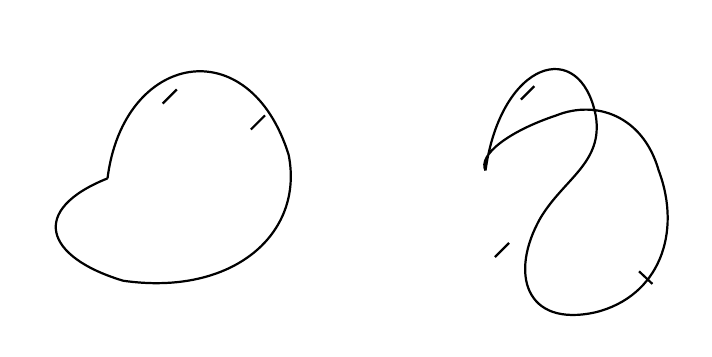
\begin{tikzpicture}[scale=1.0]
\draw[line width=0.8pt] (0,0)
  .. controls (0.2,1.6) and (1.8,1.9) .. (2.3,0.3)
  .. controls (2.5,-0.7) and (1.6,-1.5) .. (0.2,-1.3)
  .. controls (-0.8,-1.0) and (-1.0,-0.4) .. (0,0);
\draw[line width=0.8pt] (0.70,0.95) -- (0.88,1.13);
\draw[line width=0.8pt] (1.82,0.62) -- (2.00,0.80);

\draw[line width=0.8pt] (4.8,0.1)
  .. controls (5.0,1.5) and (6.0,1.8) .. (6.2,0.8)
  .. controls (6.3,0.2) and (5.8,0.0) .. (5.5,-0.5)
  .. controls (5.1,-1.2) and (5.3,-1.9) .. (6.2,-1.7)
  .. controls (7.0,-1.5) and (7.3,-0.7) .. (7.0,0.1)
  .. controls (6.8,0.8) and (6.2,1.0) .. (5.7,0.8)
  .. controls (5.1,0.6) and (4.7,0.3) .. (4.8,0.1);
\draw[line width=0.8pt] (5.25,1.00) -- (5.42,1.17);
\draw[line width=0.8pt] (5.10,-0.82) -- (4.92,-1.00);
\draw[line width=0.8pt] (6.75,-1.18) -- (6.92,-1.34);
\end{tikzpicture}
\caption{Eine klare Neuzeichnung des Kreises und der verformten Schleife. Gleicher Umfang bedeutet gleiche intrinsische eindimensionale Geometrie.}
\label{fig:c04-intrinsic-redraw}
\end{figure}

\begin{classroomqa}
\audiencequestion{Wäre ein endliches Liniensegment dieselbe Art eindimensionaler Raum?}
\lecturerresponse{Nein. Ein Segment hat zwei Endpunkte, eine geschlossene Schleife dagegen keinen. Dieser topologische Unterschied ist intrinsisch und lässt sich nicht dadurch beseitigen, dass man eines der beiden Objekte in einem größeren Raum biegt. Bei festgelegter Topologie wird das Segment durch seine Länge und die geschlossene Schleife durch ihren Umfang charakterisiert. \lecturetimestamp{00:26:00--00:26:39}}
\end{classroomqa}

\subsection{Warum Einbettungen nützlich, aber nicht erforderlich sind}

Wir veranschaulichen einen eindimensionalen Kreis, indem wir ihn in zwei Dimensionen einbetten, und eine zweidimensionale Kugel, indem wir sie in drei Dimensionen einbetten. Dieses Muster verleitet dazu, für die Diskussion einer Dreisphäre eine vierte euklidische Dimension zu verlangen. Das ist eine Folge unserer menschlichen Vorstellungskraft, keine mathematische Notwendigkeit. Unser Vorstellungsvermögen hat sich für die Orientierung in drei Dimensionen entwickelt; mit Koordinaten und Metriken können wir über diese Grenze hinaus denken, ohne einen tatsächlichen äußeren Standpunkt zu konstruieren.

\begin{classroomqa}
\audiencequestion{Könnten zusätzliche räumliche Dimensionen existieren, aber zu klein sein, um sie zu sehen?}
\lecturerresponse{Ja. Die Geometrie verlangt nicht, dass alle Dimensionen dieselbe beobachtbare Ausdehnung haben. Eine kompakte Dimension könnte viel kleiner sein als die Skalen, die gewöhnliche Erfahrungen erschließen. Der unmittelbare Punkt ist jedoch einfacher: Ob zusätzliche Dimensionen physikalisch existieren oder nicht, für die Definition der intrinsischen Metrik unseres dreidimensionalen Raumes ist keine Einbettungsdimension erforderlich. \lecturetimestamp{00:29:55--00:30:12}}
\end{classroomqa}

\begin{classroomqa}
\audiencequestion{Woran könnte ein Bewohner, der auf eine gekrümmte Linie beschränkt ist, erkennen, ob die Linie gebogen ist?}
\lecturerresponse{Allein anhand intrinsischer Messungen könnte er es nicht erkennen. Stellen wir uns Licht und Materie vor, die auf eine optische Faser beschränkt sind. Wird die Faser gebogen, ohne sie zu dehnen, ändert sich die Einbettung, nicht aber die Abstände oder Signallaufzeiten, die entlang der Faser gemessen werden. Nur ein Signal, das in den umgebenden Raum entweicht, könnte die äußere Biegung offenbaren. \lecturetimestamp{00:30:15--00:31:14}}
\end{classroomqa}

Das Gedankenexperiment lässt sich praktisch formulieren. Ein auf die Faser beschränktes Wesen könnte ein Signal aussenden, etwa ein hinreichend energiereiches Photon, und eine äußere Richtung nur dann entdecken, wenn das Signal die Faser verlässt und später auf einem Weg zurückkehrt, der innerhalb der eindimensionalen Metrik nicht verfügbar ist. In diesem Sinne ist auch die Aussage, dass der gewöhnliche Raum drei große Dimensionen hat, letztlich experimentell begründet und keine Schlussfolgerung aus dem, was sich der menschliche Geist vorstellen kann.

\begin{classroomqa}
\audiencequestion{Wenn jeder eindimensionale Raum lokal flach ist, muss dann auch jeder zweidimensionale Raum lokal flach sein?}
\lecturerresponse{Nein. Ein zu einem Zylinder gerolltes Blatt bleibt intrinsisch flach: Es lässt sich ohne Dehnung wieder abrollen. Eine Halbkugel kann dagegen nicht ohne Dehnung oder Reißen auf eine Ebene abgeflacht werden; sie besitzt intrinsische Krümmung. Jede hinreichend kleine Fläche sieht annähernd euklidisch aus, doch auf einer endlichen Skala treten messbare Abweichungen auf. Der Unterschied zwischen Zylinder und Kugel ist genau der zwischen extrinsischer Biegung und intrinsischer Krümmung. \lecturetimestamp{00:31:14--00:35:00}}
\end{classroomqa}

\begin{classroomqa}
\audiencequestion{Bedeutet intrinsische Krümmung zwangsläufig, dass ein Gravitationsfeld vorhanden ist?}
\lecturerresponse{In der allgemeinen Relativitätstheorie ist die Raumzeitkrümmung die invariante Erscheinungsform der Gezeitenwirkung der Gravitation. Die kosmologische räumliche Krümmung \(k/a^2\) gehört daher zur Gravitationsgeometrie und ist nicht bloß eine Biegung in einem vorgestellten äußeren Raum. Materie beeinflusst die Krümmung über die Einsteinsche Gleichung. Die Aussage sollte jedoch nicht zugespitzt werden zu „Krümmung gibt es nur dort, wo Materie sitzt“: Auch eine Vakuumraumzeit kann Weyl-Krümmung aufweisen, etwa außerhalb eines Sterns oder in einer Gravitationswelle. \lecturetimestamp{00:35:01--00:35:51}}
\end{classroomqa}

Nun führen wir die großräumige Idealisierung ein. Wir mitteln über Sterne, Galaxien, Galaxienhaufen und lokale Unregelmäßigkeiten, so wie man Berge außer Acht lässt, wenn man die Erde als rund beschreibt. Die resultierende räumliche Geometrie nehmen wir als homogen und isotrop an. Unter diesen Annahmen gibt es drei Möglichkeiten mit konstanter Krümmung: flach, sphärisch und hyperbolisch.

\section{Der FRW-Ansatz und die drei Krümmungsfälle}

Die Symmetrieannahmen reduzieren die Geometrie auf eine zeitabhängige Skala und ein diskretes Krümmungsvorzeichen. In mitbewegten Koordinaten lautet der Friedmann-Robertson-Walker-Ansatz
\begin{equation}
ds^2=-dt^2+a(t)^2\,d\Sigma_k^2,
\qquad
k\in\{-1,0,+1\}.
\label{eq:c04-frw}
\end{equation}
Die Zeitkoordinate ist die Eigenzeit mitbewegter Beobachter. Aufgrund der Homogenität darf \(a\) von der Zeit, nicht aber vom Ort abhängen; die Isotropie schließt eine ausgezeichnete räumliche Richtung aus.

\begin{figure}[htbp]
\centering
\includegraphics[width=0.74\textwidth]{lecture_04_figure_02.png}
\caption{Die drei räumlichen Metriken mit konstanter Krümmung, angeordnet unter dem gemeinsamen Skalenfaktor. Das Bild wurde später aufgenommen, als sich weiteres Material auf der Tafel angesammelt hatte; es bewahrt jedoch die Metrikdiskussion aus 00:40:23--00:42:42.}
\label{fig:c04-frw-board}
\lectureframe{00:45:48.386}
\end{figure}

Mit einer Radialkoordinate \(r\) und der Metrik der Einheitssphäre \(d\Omega_2^2\) lauten die drei normierten räumlichen Metriken
\begin{align}
d\Sigma_0^2 &= dr^2+r^2d\Omega_2^2,
&& k=0,
\label{eq:c04-flat-space}\\
d\Sigma_{+1}^2 &= dr^2+\sin^2 r\,d\Omega_2^2,
&& k=+1,
\label{eq:c04-spherical-space}\\
d\Sigma_{-1}^2 &= dr^2+\sinh^2 r\,d\Omega_2^2,
&& k=-1.
\label{eq:c04-hyperbolic-space}
\end{align}
Zu einer festen Zeit ist der Raum also flach, positiv oder negativ gekrümmt. Die Multiplikation mit \(a(t)^2\) verändert alle räumlichen Abstände um denselben Faktor und erhält dabei die normierte Form.

Betrachten wir zwei Galaxien mit festem mitbewegtem Abstand \(\Delta\chi\). Ihr physikalischer Abstand ist
\begin{equation}
D(t)=a(t)\Delta\chi.
\end{equation}
Durch Differenzieren und Eliminieren von \(\Delta\chi\) erhalten wir
\begin{equation}
\dot D=\dot a\,\Delta\chi
      =\frac{\dot a}{a}D
      =H(t)D,
\qquad
H(t)\equiv\frac{\dot a}{a}.
\label{eq:c04-hubble-law}
\end{equation}
Das Hubble-Gesetz folgt somit rein kinematisch aus der homogenen Skalierung. Der Hubble-Parameter kann sich mit der Zeit ändern, ist aber zu jeder festen kosmischen Zeit überall gleich.

\section{Von der Einsteinschen Gleichung zur Friedmann-Gleichung}

Die Metrik legt fest, wie Abstände gemessen werden, aber nicht, wie sich \(a(t)\) entwickelt. Für gekrümmte Raumzeit brauchen wir die Einsteinsche Gleichung. Eine Berechnung sämtlicher Christoffelsymbole und Krümmungskomponenten würde das physikalische Argument verschleiern; daher verwenden wir die durch Symmetrie vorgegebene Form und betrachten ihre Zeit-Zeit-Komponente.

In Einheiten mit \(c=1\) und vorübergehend ohne kosmologische Konstante lautet die vollständige Tensorgleichung
\begin{equation}
G_{\mu\nu}
\equiv
R_{\mu\nu}-\frac12 g_{\mu\nu}R
=8\pi G\,T_{\mu\nu}.
\label{eq:c04-einstein}
\end{equation}
Auf der linken Seite steht die Geometrie, auf der rechten Energiedichte, Impulsdichte, Druck und Spannung. Der Faktor \(1/3\) gehört nicht in die vollständige Tensorgleichung. Er tritt erst auf, nachdem die Zeit-Zeit-Komponente auf die Friedmann-Form reduziert wurde.

\begin{figure}[htbp]
\centering
\includegraphics[width=0.78\textwidth]{lecture_04_figure_03.png}
\caption{Ein Zwischenstand der Tafel zur Einsteinschen Gleichung. Die geometrische linke Seite ist zu sehen, während der Materietensor noch nicht lesbar und die dargestellte Normierung unvollständig ist. Gleichung~\eqref{eq:c04-einstein} hält die übliche vollständige Tensorgleichung fest, die in der Herleitung verwendet wird.}
\label{fig:c04-einstein-board}
\lectureframe{00:48:19.394}
\end{figure}

Für ein homogenes Fluid in Ruhe in mitbewegten Koordinaten gilt
\begin{equation}
T_{00}=\rho.
\label{eq:c04-energy-density}
\end{equation}
Der Zeit-Zeit-Komponente des Einstein-Tensors kommt eine nützliche strukturelle Eigenschaft zu. Die Ableitungen zweiter Ordnung heben sich auf; übrig bleiben ein Term quadratisch in der ersten Zeitableitung und ein Term aufgrund der räumlichen Krümmung:
\begin{equation}
G_{00}=3\left[
\left(\frac{\dot a}{a}\right)^2+\frac{k}{a^2}
\right].
\label{eq:c04-g00}
\end{equation}
Durch Einsetzen der Gleichungen ~\eqref{eq:c04-energy-density} und \eqref{eq:c04-g00} in Gleichung ~\eqref{eq:c04-einstein} erhalten wir die erste Friedmann-Gleichung:
\begin{equation}
\boxed{
\left(\frac{\dot a}{a}\right)^2+\frac{k}{a^2}
=\frac{8\pi G}{3}\rho
}.
\label{eq:c04-friedmann}
\end{equation}
Äquivalent dazu gilt
\begin{equation}
H^2=\frac{8\pi G}{3}\rho-\frac{k}{a^2}.
\label{eq:c04-friedmann-energy}
\end{equation}
Gleichung ~\eqref{eq:c04-friedmann-energy} hat genau die Form, die wir schon im früheren Newtonschen Argument gefunden haben. Dort wurde die Integrationskonstante als Gesamtenergie oder Fluchtbedingung einer Materiekugel gedeutet. In der allgemeinen Relativitätstheorie nimmt die intrinsische räumliche Krümmung denselben mathematischen Platz ein. Diese Übereinstimmung ist kein Zufall: In einem hinreichend kleinen Gebiet werden Krümmungseffekte vernachlässigbar, und die relativistische Kosmologie muss das lokale Newtonsche Verhalten wiedergeben. Die Relativitätstheorie macht außerdem deutlich, dass \(\rho\) die Gesamtenergiedichte bezeichnet. Daher gravitieren auch relativistische Teilchen und Photonen, obwohl ein Argument, das nur von nichtrelativistischer Massendichte ausgeht, sie nicht erfassen würde.

\begin{classroomqa}
\audiencequestion{Warum gibt es in der Metrik keine Terme, die Raum und Zeit mischen?}
\lecturerresponse{Ein gemischter Term entspräche einem ausgezeichneten räumlichen Vektor oder einer Strömung relativ zu den mitbewegten Beobachtern. Exakte Homogenität und Isotropie lassen keine solche Richtung zu. In Koordinaten, die an die kosmische Materie angepasst sind, verschwindet daher der Verschiebungsvektor, und die Metrik nimmt die Blockdiagonalform aus Gleichung ~\eqref{eq:c04-frw} an. Sind die angenommenen Symmetrien gewahrt, ist das keine zusätzliche dynamische Vermutung, sondern ihre geometrische Folge. \lecturetimestamp{00:58:27--00:59:08}}
\end{classroomqa}

\begin{classroomqa}
\audiencequestion{Warum genügt die Zeit-Zeit-Komponente, und wohin verschwinden die Ableitungen zweiter Ordnung?}
\lecturerresponse{Der homogene und isotrope Ansatz enthält nur eine unbekannte Funktion, \(a(t)\). Die gemischten Komponenten reduzieren sich auf Identitäten, während die räumlichen Komponenten mit der Zeit-Zeit-Gleichung und der Erhaltung des Energie-Impuls-Tensors zusammenhängen. Man kann sie mit der Zeit-Zeit-Gleichung zu einer Beschleunigungsgleichung mit \(\ddot a\) kombinieren; die Zeit-Zeit-Komponente des Einstein-Tensors ist jedoch besonders: Ihre Terme mit Ableitungen zweiter Ordnung heben sich auf, sodass die Energiegleichung erster Ordnung ~\eqref{eq:c04-friedmann} übrig bleibt. Eine nichttriviale Gleichung zusammen mit dem Entwicklungsgesetz für die Materie reicht aus, um den einen geometrischen Freiheitsgrad zu bestimmen. \lecturetimestamp{00:59:09--01:00:56}}
\end{classroomqa}

\section{Wie der Inhalt des Universums verdünnt wird}

Die Friedmann-Gleichung ist erst dann vollständig, wenn \(\rho\) als Funktion von \(a\) bekannt ist. Die Geometrie hat eine Gleichung geliefert; die Materie im Universum muss die zweite Beziehung beisteuern.

Bei nichtrelativistischer Materie bleibt die Teilchenzahl in einem mitbewegten Volumen konstant, während das physikalische Volumen wie \(a^3\) anwächst. Vernachlässigen wir die geringe kinetische Energie der Teilchen, so gilt
\begin{equation}
\rho_{\mathrm m}(a)=\frac{\rho_{\mathrm m,0}}{a^3}.
\label{eq:c04-matter-scaling}
\end{equation}
Die Normierung \(a=1\) kann hier für eine beliebige zweckmäßige Referenzepoche gewählt werden; unmittelbar bedeutsam sind nur Verhältnisse von Skalenfaktoren.

\begin{classroomqa}
\audiencequestion{Wenn ein flaches Universum unendlich ist, was bedeutet es dann, dass \(a\) zum Urknall hin gegen null geht?}
\lecturerresponse{Ein unendlicher flacher Raum bleibt für jeden von null verschiedenen Wert von \(a\) unendlich; alle endlichen mitbewegten Abstände werden mit demselben schrumpfenden Faktor multipliziert. Im flachen Fall ist die absolute Normierung von \(a\) beliebig, sodass nur \(a(t_2)/a(t_1)\) eine invariante Bedeutung hat. Für ein geschlossenes sphärisches Universum ist \(a\) natürlicherweise sein Krümmungsradius; für ein hyperbolisches Universum legt es den Krümmungsradius fest. Der Grenzfall \(a\to0\) kennzeichnet die kosmologische Singularität und keine gewöhnliche endliche Kugel in einem äußeren Raum. \lecturetimestamp{01:05:06--01:05:53}}
\end{classroomqa}

Strahlung verliert auf zwei Arten Energie. Ihre Teilchendichte nimmt umgekehrt proportional zum Volumen ab, und die Wellenlänge jedes Photons wird proportional zu \(a\) gedehnt, wodurch sich seine Energie um einen weiteren Faktor \(a^{-1}\) verringert. Daher gilt
\begin{equation}
\rho_{\mathrm r}(a)=\frac{\rho_{\mathrm r,0}}{a^4}.
\label{eq:c04-radiation-scaling}
\end{equation}
Da \(a^{-4}\) bei einer Rückentwicklung in die Vergangenheit schneller anwächst als \(a^{-3}\), dominiert Strahlung in hinreichend frühen Zeiten, selbst wenn viel später Materie dominiert.

Wären Materie und Strahlung die einzigen Bestandteile, würde das Vorzeichen von \(k\) die Zukunft weitgehend bestimmen: \(k=+1\) erlaubt einen erneuten Kollaps, \(k=0\) ist der Grenzfall, der sich ewig, aber zunehmend langsamer ausdehnt, und \(k=-1\) führt zu ewiger Expansion, bei der die Krümmung schließlich wichtig wird. Dunkle Energie hebt diesen einfachen Zusammenhang auf. Ein geschlossenes Universum kann sich ewig ausdehnen, und aus räumlicher Flachheit allein lässt sich das endgültige Schicksal nicht ableiten.

\section{Zustandsgleichung und Kontinuitätsgleichung}

Anstatt für jeden Stoff eine eigene Verdünnungsregel auswendig zu lernen, beschreiben wir die Materie durch eine Zustandsgleichung. Das Vorgehen hat zwei Teile. Zuerst leiten wir \(\rho(a)\) für eine gegebene Beziehung zwischen Druck und Energiedichte her. Dann bestimmen wir diese Beziehung aus der mikroskopischen Physik von Materie, Strahlung oder Vakuum. Für die vorliegende Vorlesung genügt der erste Teil.

Druck ist Impulsfluss. Moleküle, die auf die Wand eines Kastens treffen, kehren ihren Impuls um und üben eine Kraft auf die Wand aus; schnellere Teilchen übertragen mehr Impuls und erzeugen einen höheren Druck. Sind die Art des Stoffes und seine Eigenschaften festgelegt, lassen sich Energiedichte und Druck daher nicht unabhängig voneinander wählen. Für eine einfache kosmologische Komponente schreiben wir
\begin{equation}
P=w\rho,
\label{eq:c04-equation-state}
\end{equation}
Dabei ist \(w\) in Einheiten mit \(c=1\) dimensionslos. Kalte Materie hat vernachlässigbaren Druck und damit \(w=0\). Für Strahlung gilt \(w=1/3\); der Faktor \(1/3\) ergibt sich aus der Mittelung über die drei räumlichen Richtungen.

\begin{figure}[htbp]
\centering
\includegraphics[width=0.82\textwidth]{lecture_04_figure_06.png}
\caption{Die Tafel fasst die Skalierungen für Materie und Strahlung zusammen und schreibt die Zustandsgleichung als \(P=W\rho\). Wir verwenden das übliche kleine \(w\).}
\label{fig:c04-equation-state-board}
\lectureframe{01:15:08.166}
\end{figure}

\subsection{Thermodynamik in einem mitbewegten Kasten}

Betrachten wir einen mitbewegten Kasten mit physikalischem Volumen \(V\) und Energiedichte \(\rho\) sowie der Gesamtenergie
\begin{equation}
E=\rho V.
\end{equation}
Der erste Hauptsatz lautet
\begin{equation}
dE=T\,dS-P\,dV.
\end{equation}
Die kosmologische Expansion wird als adiabatisch behandelt, sodass für den mitbewegten Kasten \(dS=0\) gilt und
\begin{equation}
dE=-P\,dV.
\label{eq:c04-adiabatic-first-law}
\end{equation}
Das Minuszeichen bedeutet, dass ein expandierendes System Arbeit verrichtet und innere Energie verliert. Leiten wir \(E=\rho V\) unabhängig davon ab, so erhalten wir
\begin{equation}
dE=\rho\,dV+V\,d\rho.
\end{equation}
Durch Gleichsetzen der beiden Ausdrücke folgt
\begin{align}
\rho\,dV+V\,d\rho&=-P\,dV,\\
V\,d\rho&=-(\rho+P)\,dV.
\label{eq:c04-volume-continuity}
\end{align}
Mit \(P=w\rho\) gilt
\begin{equation}
\frac{d\rho}{\rho}=-(1+w)\frac{dV}{V}.
\end{equation}
Integration liefert
\begin{equation}
\rho\propto V^{-(1+w)}.
\end{equation}
Da ein mitbewegtes Volumen wie \(V\propto a^3\) skaliert, gilt
\begin{equation}
\boxed{\rho(a)\propto a^{-3(1+w)}}.
\label{eq:c04-density-scaling}
\end{equation}
In Differentialform lautet dieselbe Aussage die lokale Energieerhaltungsgleichung
\begin{equation}
\dot\rho+3H(\rho+P)=0.
\label{eq:c04-continuity}
\end{equation}
Dieses lokale Erhaltungsgesetz gilt weiterhin exakt, obwohl eine sich verändernde kosmologische Geometrie keine global erhaltene Gesamtenergie voraussetzt.

Die beiden bekannten Fälle folgen unmittelbar:
\begin{align}
w=0
&\quad\Longrightarrow\quad
\rho_{\mathrm m}\propto a^{-3},\\
w=\frac13
&\quad\Longrightarrow\quad
\rho_{\mathrm r}\propto a^{-4}.
\end{align}
Der zusätzliche inverse Faktor bei der Strahlung ist der thermodynamische Ausdruck der kosmologischen Rotverschiebung.

\begin{classroomqa}
\audiencequestion{Welche Strahlung ist heute noch im Universum vorhanden?}
\lecturerresponse{In der Vorlesung geht es dabei vor allem um die kosmische Mikrowellenhintergrundstrahlung, das Reliktphotonenbad aus dem heißen frühen Universum. Strahlung macht heute nur einen kleinen Teil der gesamten kosmischen Energiedichte aus; wegen ihrer Skalierung \(a^{-4}\) überwiegt sie jedoch die Materie, wenn man die Gleichungen weit genug in die Vergangenheit zurückverfolgt. Die genauen heutigen Anteile sind Beobachtungsgrößen und für dieses Skalierungsargument nicht erforderlich. \lecturetimestamp{01:26:53--01:28:34}}
\end{classroomqa}

\section{Vakuumenergie und das Scheitern der Krümmungsregel für das Schicksal des Universums}

Dunkle Energie führt zur Zustandsgleichung
\begin{equation}
P=-\rho,
\qquad
w=-1.
\label{eq:c04-vacuum-eos}
\end{equation}
Negativer Druck ist eine Zugspannung: Statt gegen die Wand eines Kastens nach außen zu drücken, zieht der Inhalt sie nach innen. Eine gespannte Feder ist ein vertrautes Beispiel für Zugspannung, allerdings nur eine Analogie und kein mikroskopisches Modell der Vakuumenergie.

\begin{classroomqa}
\audiencequestion{Hängt negativer Druck mit dem absoluten Nullpunkt zusammen?}
\lecturerresponse{Nicht auf einfache allgemeine Weise. Kühlt man einen gewöhnlichen Stoff auf den absoluten Nullpunkt ab, entsteht dadurch nicht von selbst die kosmologische Zustandsgleichung \(P=-\rho\). Die Frage ist nützlich, weil sie thermischen Druck von Vakuumspannung unterscheidet: Vakuumenergie ist durch einen Lorentz-invarianten Energie-Impuls-Tensor gekennzeichnet, dessen räumliche Komponenten als negativer Druck wirken. Ihr mikroskopischer Ursprung ist eine eigene Frage. \lecturetimestamp{01:31:01--01:31:46}}
\end{classroomqa}

Setzt man \(w=-1\) in Gleichung~\eqref{eq:c04-density-scaling} ein, erhält man
\begin{equation}
\rho_\Lambda\propto a^0=\text{constant}.
\label{eq:c04-vacuum-density}
\end{equation}
Wenn sich ein mitbewegtes Gebiet ausdehnt, nehmen sein Volumen und seine gesamte Vakuumenergie gemeinsam zu; die Energie pro Volumeneinheit bleibt dabei unverändert. Der Arbeitsterm in Gleichung~\eqref{eq:c04-adiabatic-first-law} trägt diesem Verhalten Rechnung, denn \(P\) ist negativ. Sobald eine solche Komponente vorhanden ist, garantiert eine positive räumliche Krümmung keinen erneuten Kollaps mehr.

\begin{classroomqa}
\audiencequestion{Welche Rolle spielen Dunkle Materie, Schwarze Löcher und andere kompakte Objekte?}
\lecturerresponse{Auf Skalen, die groß gegenüber ihren Abständen sind, gehört jede nichtrelativistische Komponente mit kleinen ungeordneten Geschwindigkeiten zur drucklosen Materiedichte. Dazu zählen gewöhnliche Materie, kalte Dunkle Materie und eine Population kompakter Objekte wie Schwarze Löcher. Ihre lokale Struktur ist kompliziert, aber nach einer Mittelung über kleine Skalen ist ihre mittlere kosmologische Zustandsgleichung näherungsweise \(w=0\). \lecturetimestamp{01:33:34--01:34:10}}
\end{classroomqa}

\begin{classroomqa}
\audiencequestion{Ergeben die relativistischen Gleichungen dieselben Lösungen für ein materie- beziehungsweise strahlungsdominiertes Universum wie zuvor?}
\lecturerresponse{Ja. Für \(k=0\) ergibt das Einsetzen von \(\rho_{\mathrm m}\propto a^{-3}\) in die Friedmann-Gleichung \(\dot a^2\propto a^{-1}\) und damit \(a(t)\propto t^{2/3}\). Setzt man \(\rho_{\mathrm r}\propto a^{-4}\) ein, erhält man \(\dot a^2\propto a^{-2}\) und \(a(t)\propto t^{1/2}\). Die Allgemeine Relativitätstheorie verändert die Interpretation und erweitert die möglichen Quellen, lässt diese Lösungen aber bestehen. \lecturetimestamp{01:34:14--01:35:12}}
\end{classroomqa}

\begin{classroomqa}
\audiencequestion{Welcher Kraft würde dunkle Energie in einem Newtonschen Bild ähneln?}
\lecturerresponse{Eine positive kosmologische Konstante bewirkt eine abstoßende Relativbeschleunigung, die proportional zum Abstand ist,
\[
\ddot D=\frac{\Lambda}{3}D
\]
in Einheiten mit \(c=1\). Eine negative kosmologische Konstante kehrt das Vorzeichen um und wirkt anziehend. Da der Effekt bei positivem \(\Lambda\) mit der Entfernung zunimmt, kann er Materie und Krümmung schließlich dominieren; dann kann sich sogar ein geschlossenes \(k=+1\)-Universum weiter ausdehnen. Diese Newtonsche Form ist lediglich ein nützliches Abbild der relativistischen Dynamik. \lecturetimestamp{01:35:13--01:36:55}}
\end{classroomqa}

\section{Was Sie mitnehmen sollten}

Das kosmologische Prinzip ist eine geometrische Aussage über gemittelte Größen: Nachdem die lokale Struktur herausgemittelt wurde, ist jeder Punkt jeder Richtung gleichwertig. Es schränkt die räumliche Metrik auf die drei Fälle konstanter Krümmung ein und fasst die gesamte Zeitabhängigkeit in \(a(t)\) zusammen:
\begin{equation}
ds^2=-dt^2+a(t)^2d\Sigma_k^2.
\end{equation}
Mitbewegte Abstände erfüllen dann \(\dot D=HD\), während gebundene Systeme dieser Strömung nicht folgen müssen.

Einsteins Gleichung für die Zeit-Zeit-Komponente macht aus dem Ansatz eine Dynamik:
\begin{equation}
H^2+\frac{k}{a^2}=\frac{8\pi G}{3}\rho.
\end{equation}
Die Ähnlichkeit mit der Newtonschen Energiegleichung ist durchaus real, doch in der Allgemeinen Relativitätstheorie wird der Integrationsparameter mit der intrinsischen räumlichen Krümmung identifiziert, und jede Energieform kann einen Beitrag leisten.

Der verbleibende Baustein ist thermodynamischer Art. Für eine adiabatisch expandierende Komponente mit \(P=w\rho\) gilt:
\begin{equation}
\dot\rho+3H(\rho+P)=0,
\qquad
\rho\propto a^{-3(1+w)}.
\end{equation}
Materie, Strahlung und Vakuumenergie entsprechen der Reihe nach
\begin{equation}
w=0,\qquad w=\frac13,\qquad w=-1.
\end{equation}
Ihre unterschiedlichen Verdünnungsraten bestimmen, welche Komponente die Expansion in jeder Epoche beherrscht. Als Nächstes gilt es, die Physik hinter diesen Zustandsgleichungen und der durch Vakuumenergie verursachten Beschleunigung zu verstehen.
